\documentclass[conference]{IEEEtran}

\usepackage{amsmath,amssymb}
\usepackage{booktabs}
\usepackage{cite}
\usepackage{graphicx}
\usepackage[hidelinks]{hyperref}

\title{Microchip Character Recognition Using Image Processing and Machine Learning}

\author{
  \IEEEauthorblockN{Group 8}
  \IEEEauthorblockA{
    ME5411 Robot Vision and AI\\
    National University of Singapore\\
    Singapore
  }
}

\begin{document}

\maketitle

\begin{abstract}
This report presents an image-processing and machine-learning pipeline for
recognizing characters printed on a microchip. The final report will describe
the preprocessing, segmentation, feature extraction, classification, and
evaluation procedures developed by Group 8.
\end{abstract}

\begin{IEEEkeywords}
robot vision, image processing, character recognition, convolutional neural
network, classification
\end{IEEEkeywords}

\section{Introduction}
Character recognition in low-contrast industrial imagery requires careful
preprocessing, segmentation, and classification. Classical image-processing
methods provide interpretable tools for enhancing and isolating characters
\cite{gonzalez2018digital}, while convolutional neural networks can learn
features directly from image data \cite{lecun1998gradient}.

The implementation is organised as six reproducible tasks. Tasks 1--4 use
classical image-processing operators covered in the lectures; Tasks 5 and 6
compare a compact CNN with a conventional HOG-based classifier. Since the
course images are kept outside the repository, numerical results are generated
by the supplied commands after the data are placed in \texttt{data/raw/}.

\section{Problem Formulation}
Describe the input image, recognition targets, operating assumptions, and
evaluation criteria. State the dataset split and measures used for comparison.

\section{Methodology}

\subsection{Image Enhancement and Smoothing}

\subsubsection{Task 1: Image Enhancement}

Task 1 aims to improve the legibility of the characters printed on the
microchip. In the input image, the characters have intensities similar to
those of the background, while the prominent background texture further
reduces their visibility. The image is first converted into an 8-bit
grayscale representation. Contrast stretching and histogram equalization
are then applied separately to investigate their effects on image contrast
and character details.

\paragraph{Contrast Stretching}

Contrast stretching is a piecewise-linear intensity transformation that
maps the selected input intensity interval $[L,H]$ to the output range
$[0,255]$. Input intensities below $L$ are set to 0, whereas intensities
above $H$ are set to 255. For $H>L$, the transformation is defined as

\begin{equation}
g(x,y)=
\begin{cases}
0, & f(x,y)\leq L,\\[3pt]
\displaystyle 255\frac{f(x,y)-L}{H-L},
& L<f(x,y)<H,\\[6pt]
255, & f(x,y)\geq H.
\end{cases}
\label{eq:stretch}
\end{equation}

Here, $f(x,y)$ and $g(x,y)$ denote the input and output intensities at
pixel location $(x,y)$, respectively. The parameters $L$ and $H$ represent
the lower and upper limits of the selected input intensity interval.
Unless specified manually, these limits are determined from the minimum
and maximum intensities of the input image:

\begin{equation}
L=\min_{x,y}f(x,y),
\qquad
H=\max_{x,y}f(x,y).
\label{eq:stretch_limits}
\end{equation}

The mapped values are rounded to the nearest integer, clipped to the valid
range from 0 to 255, and stored as an 8-bit grayscale image. If $H\leq L$,
the implementation returns an all-zero image to avoid an invalid division.

Contrast stretching expands the intensity differences within the selected
interval. However, because the transformation does not distinguish between
character pixels and background pixels, it may also amplify background
texture. If the input image already spans the full intensity range from
0 to 255, applying the default limits produces little or no change.

\paragraph{Histogram Equalization}

Histogram equalization constructs an intensity mapping from the grayscale
distribution of the entire image. It uses the cumulative distribution
function to redistribute the intensity levels, allowing densely populated
input intensity intervals to occupy a wider output range.

Let $N$ denote the total number of pixels in the image and $n_k$ denote
the number of pixels with intensity $k$. The normalized grayscale
histogram is defined as

\begin{equation}
p(k)=\frac{n_k}{N},
\qquad k=0,1,\ldots,255.
\label{eq:normalized_histogram}
\end{equation}

The corresponding cumulative distribution function is

\begin{equation}
C(k)=\sum_{j=0}^{k}p(j),
\label{eq:histogram_cdf}
\end{equation}
where $C(k)$ represents the proportion of pixels with intensities less
than or equal to $k$.

The implementation subtracts the minimum nonzero cumulative value so
that the lowest intensity present in the image is mapped to 0. Let
$k_{\min}$ denote the lowest occupied intensity level. The corresponding
minimum cumulative value is

\begin{equation}
C_{\min}=C(k_{\min}).
\label{eq:histogram_cdf_min}
\end{equation}

For an image containing at least two distinct intensity levels, the
equalization mapping is defined as

\begin{equation}
\begin{split}
T(k)=\operatorname{clip}\Bigg(
\operatorname{round}\Bigg[
255\frac{C(k)-C_{\min}}{1-C_{\min}}
\Bigg],\,0,\,255\Bigg).
\end{split}
\label{eq:histogram_mapping}
\end{equation}

The mapping is then applied to each input pixel:

\begin{equation}
g(x,y)=T\bigl(f(x,y)\bigr).
\label{eq:histogram_output}
\end{equation}

In \eqref{eq:histogram_mapping}, $\operatorname{round}$ rounds the
calculated value to the nearest integer, whereas $\operatorname{clip}$
restricts the result to the valid 8-bit range from 0 to 255. The
implementation uses this mapping to construct a lookup table containing
256 entries and applies the table to all pixels in the input image. If
the input image contains only one intensity level, it is returned
unchanged.

Figure~\ref{fig:histogram_equalization} presents the grayscale
histograms before and after histogram equalization. Both histograms
use intensity level on the horizontal axis and pixel count on the
vertical axis. Identical axis limits are used to facilitate comparison.

\begin{figure}[!t]
    \centering

    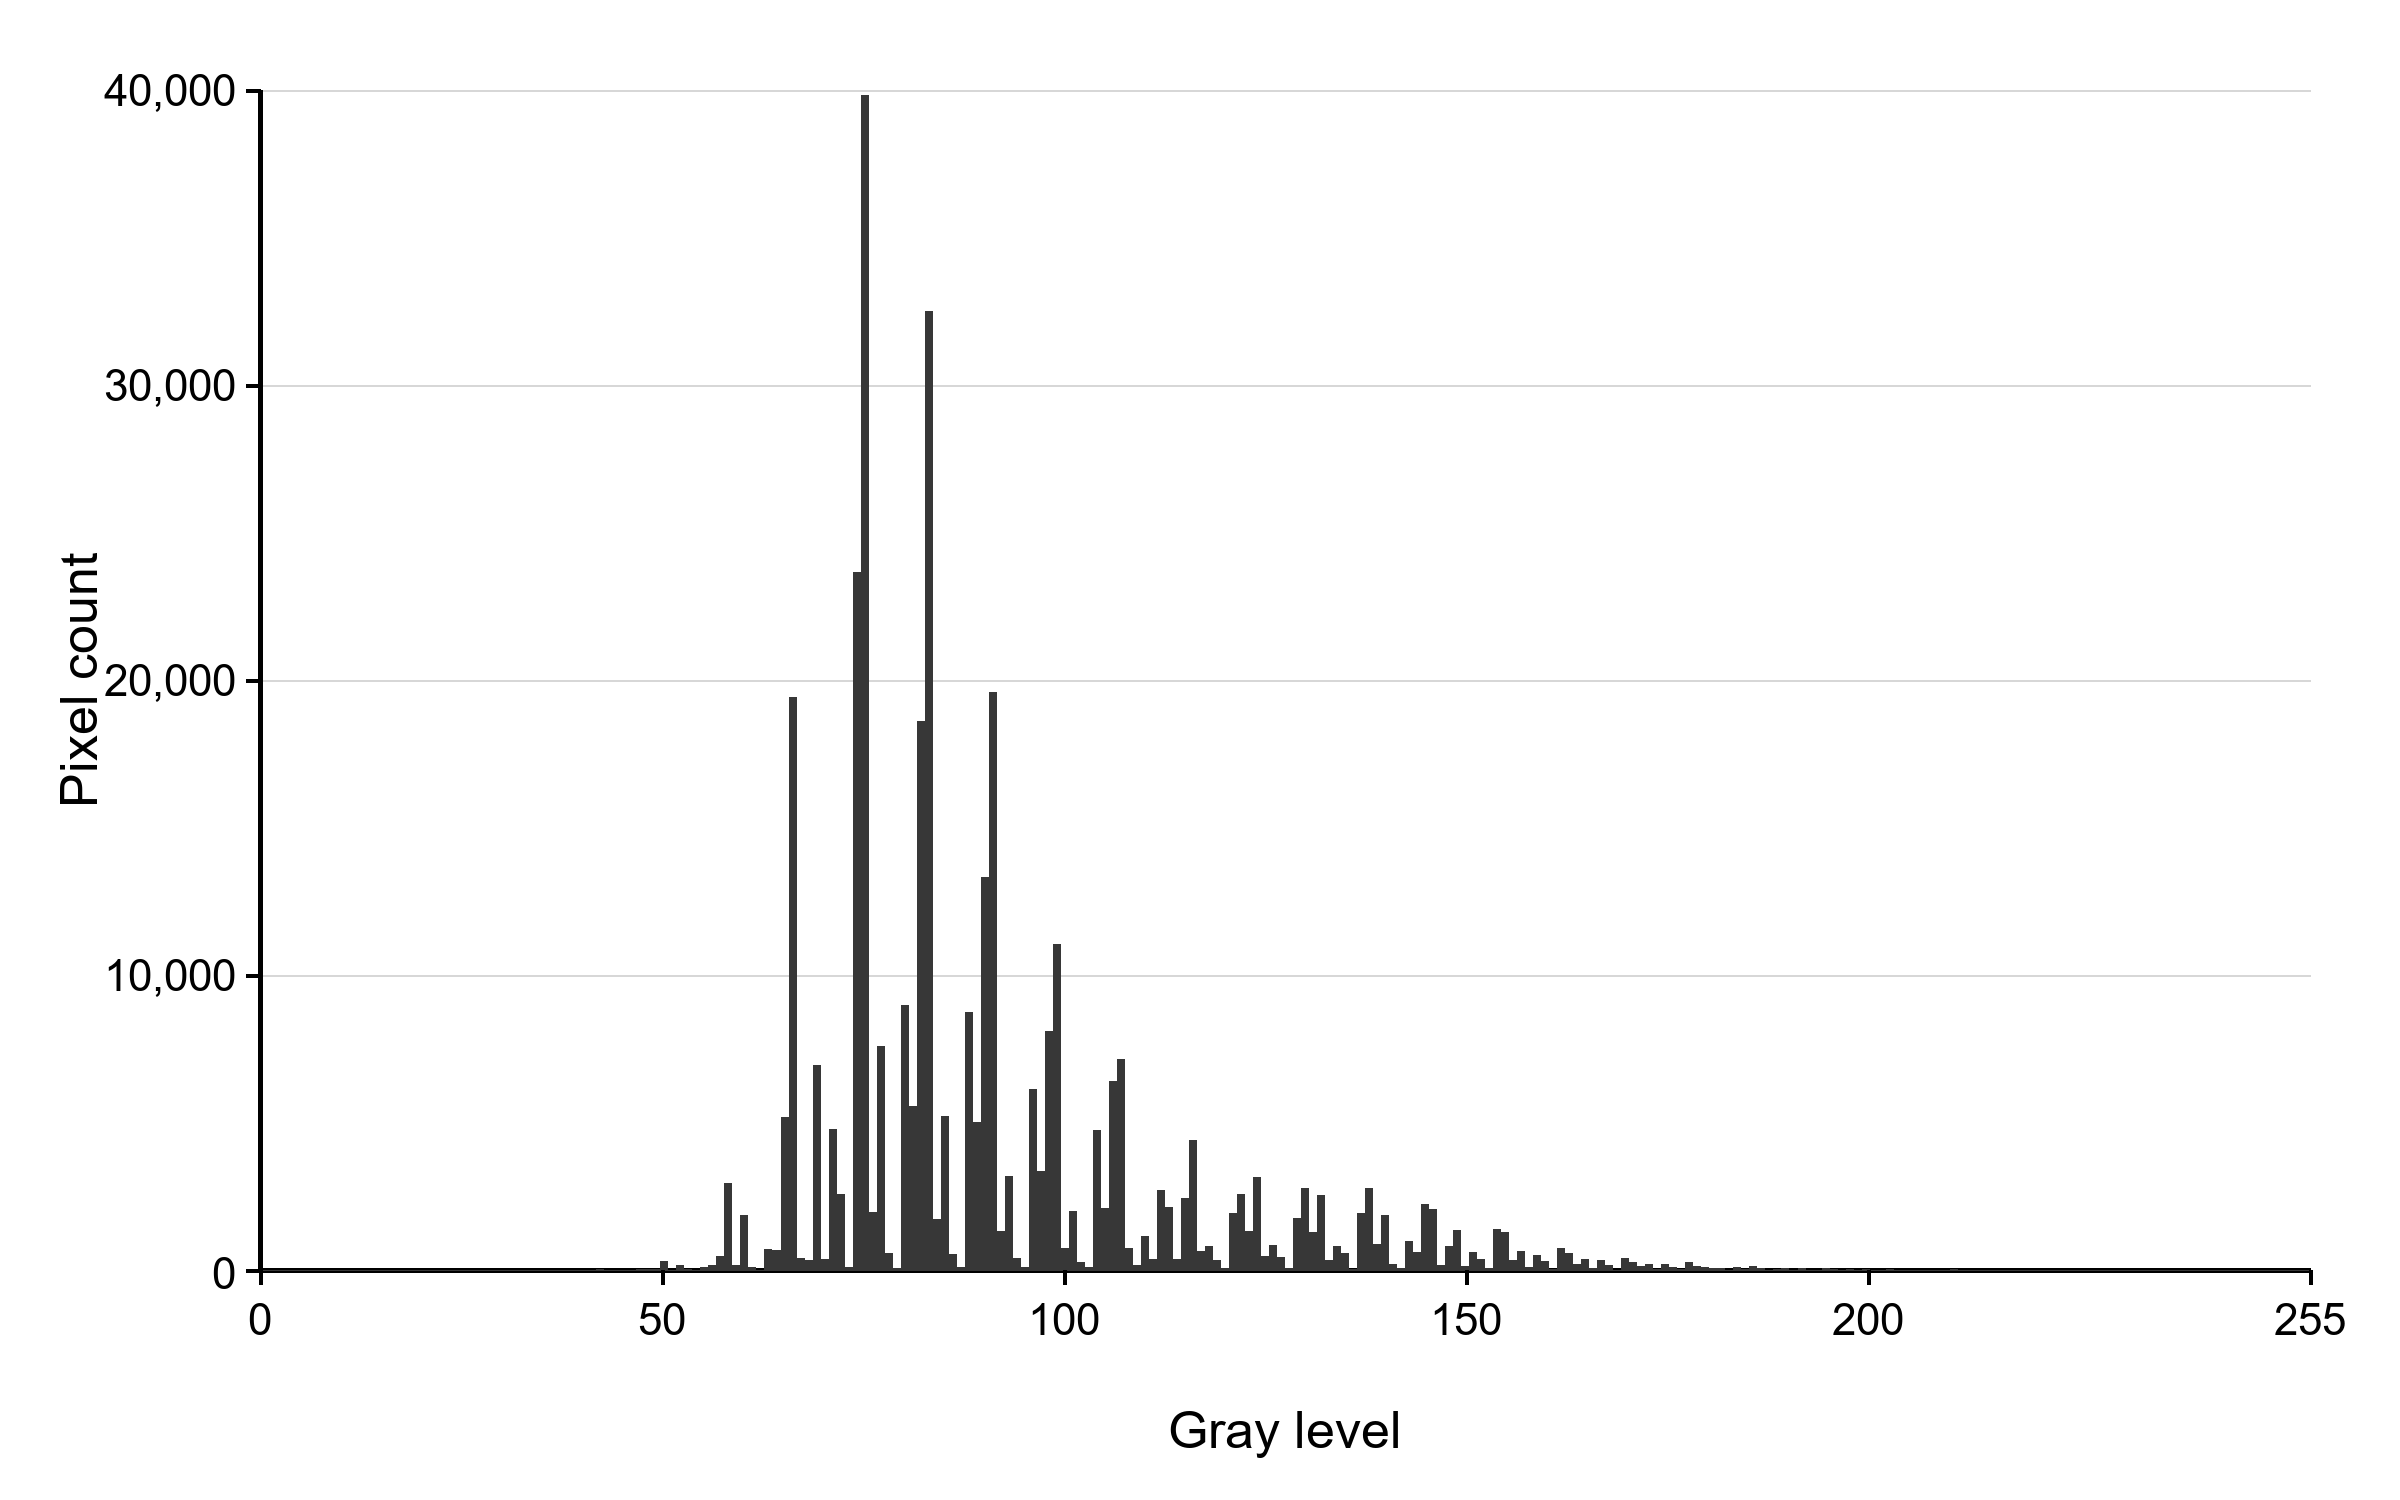
\includegraphics[width=\columnwidth]
    {histogram_original.png}

    \textnormal{(a) Original grayscale histogram}

    \vspace{1.5mm}

    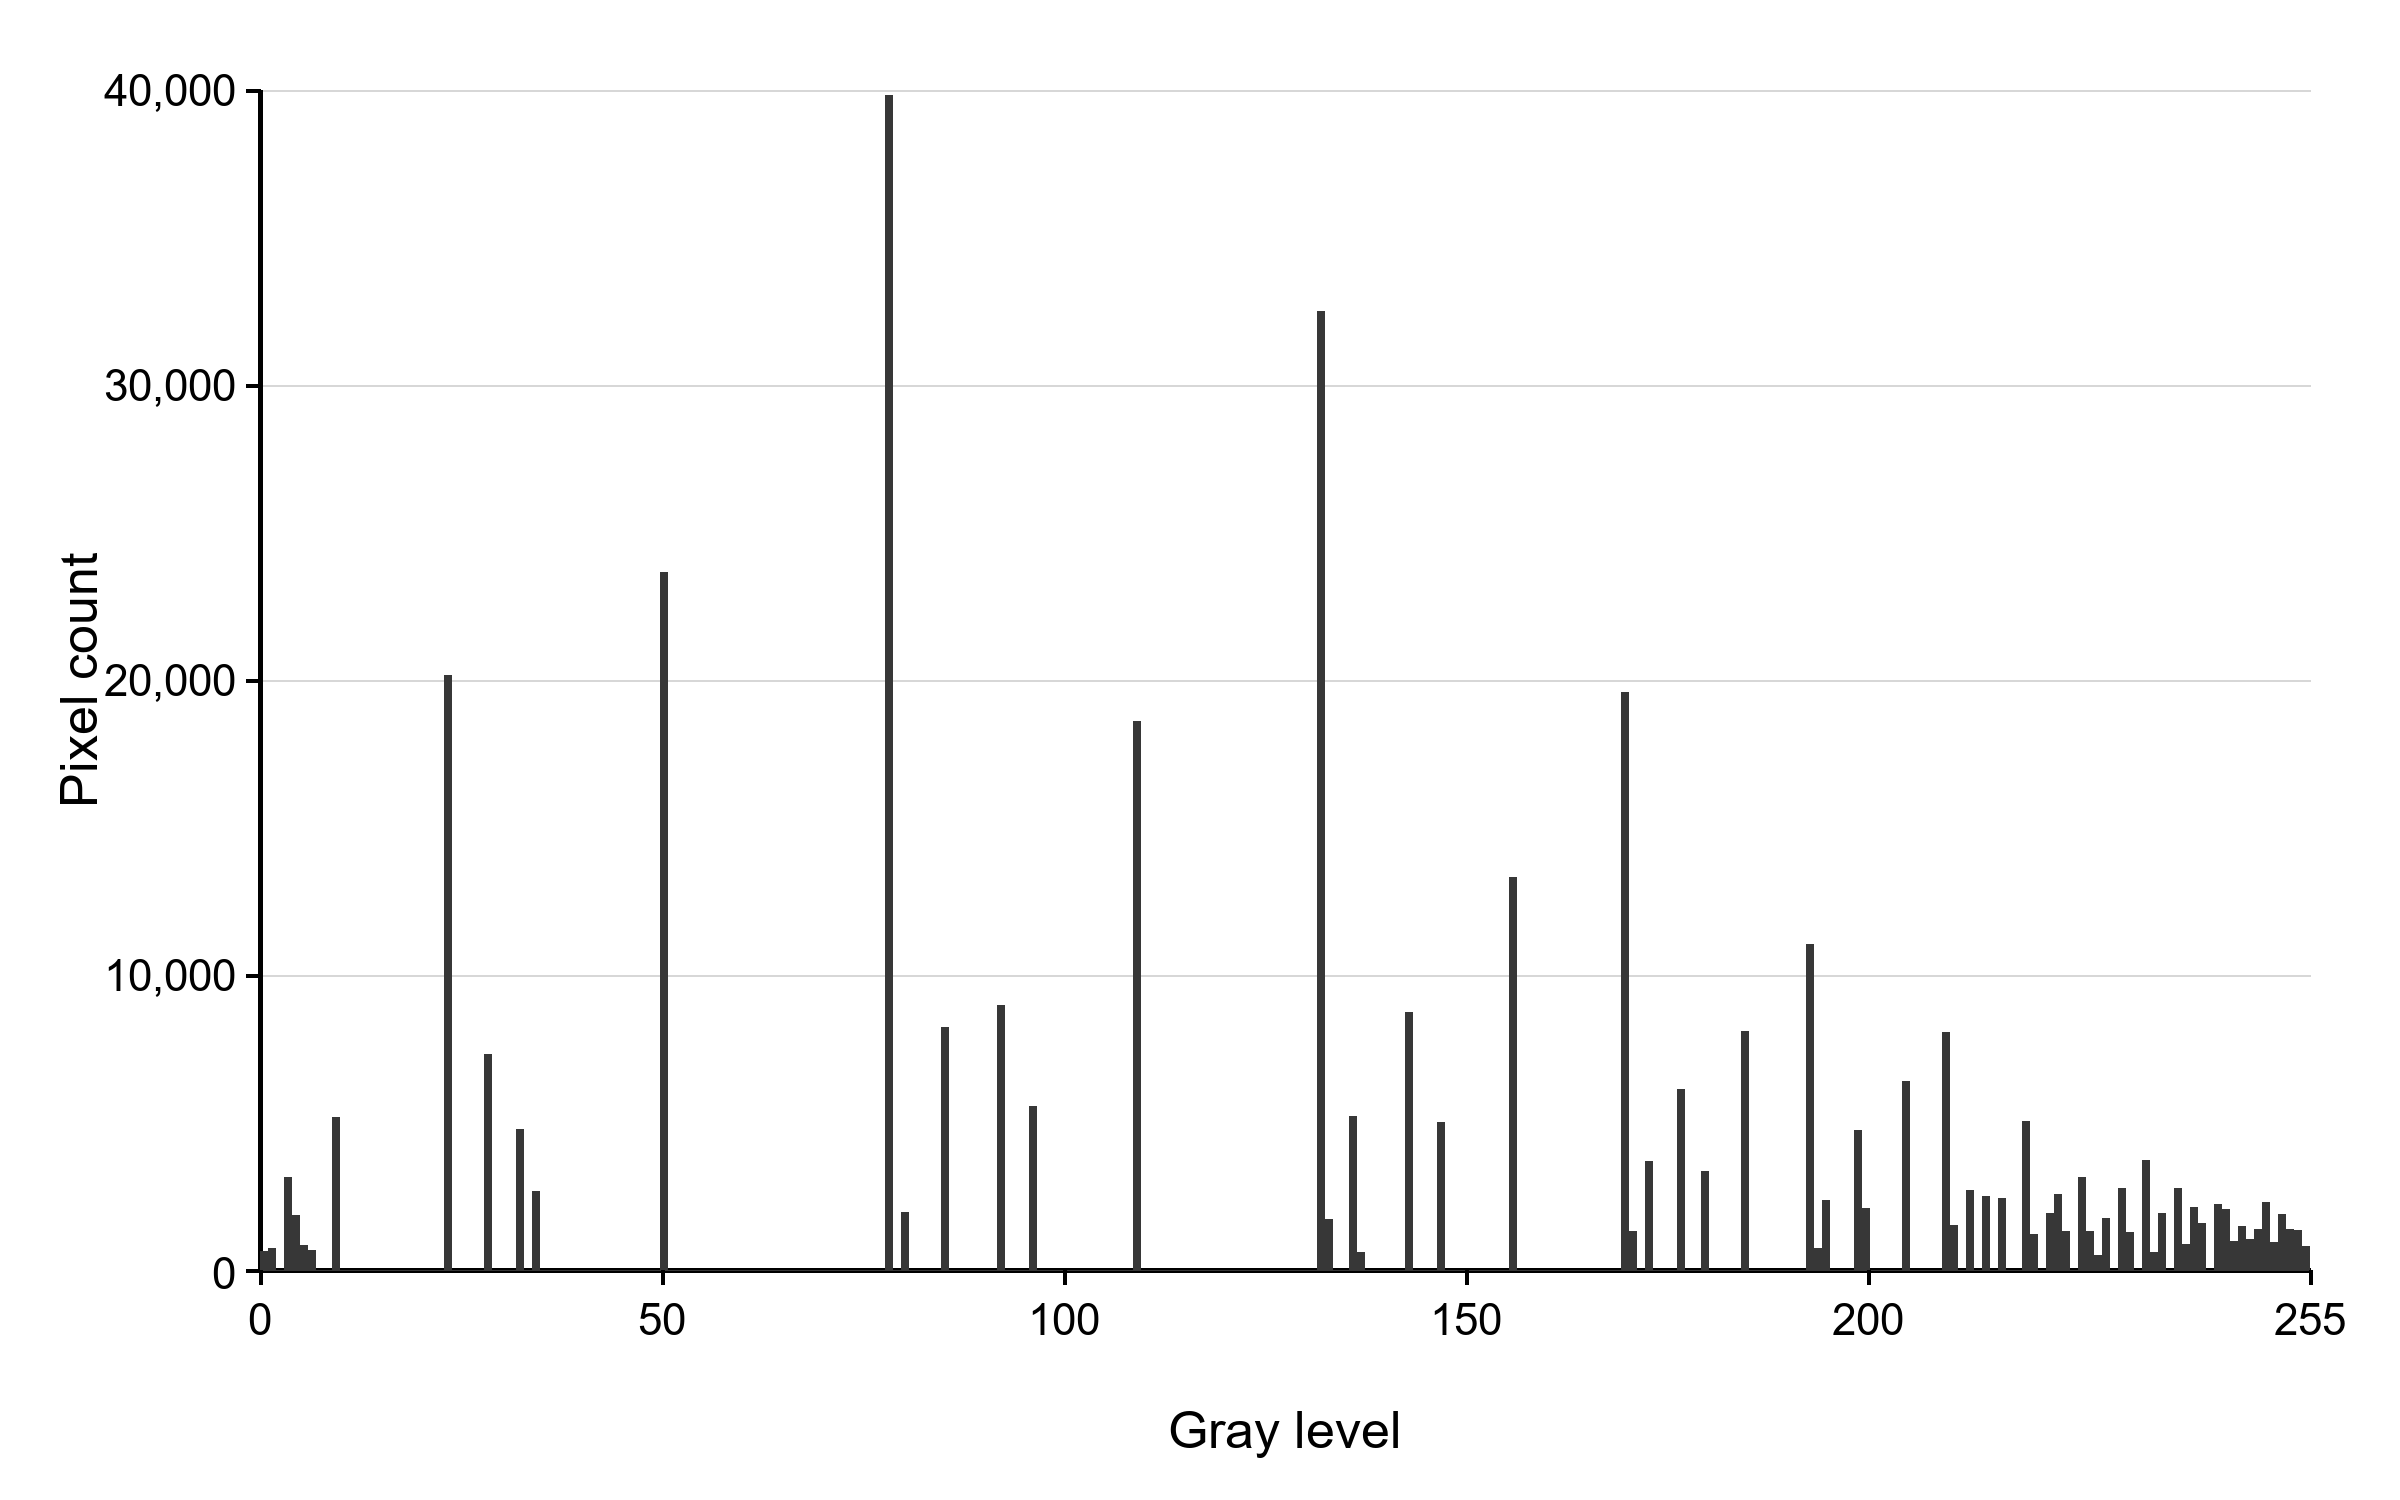
\includegraphics[width=\columnwidth]
    {histogram_equalized.png}

    \textnormal{(b) Histogram after equalization}

    \caption{Grayscale histograms before and after histogram
    equalization: (a) original grayscale histogram;
    (b) histogram after equalization.}
    \label{fig:histogram_equalization}
\end{figure}

Because digital images contain discrete intensity levels, the equalized
histogram is not necessarily perfectly uniform. Furthermore, histogram
equalization does not distinguish character pixels from background
pixels and may therefore emphasize background texture and noise while
increasing character contrast. The enhanced images and the practical
effects of both methods are evaluated in the Results and Discussion
sections.

\subsubsection{Task 2: Image Smoothing}

Task 2 applies spatial smoothing to the microchip character image. A
$5\times5$ averaging filter is first implemented as required, and
averaging filters of different sizes are subsequently compared to examine
the trade-off between suppressing background intensity variations and
preserving character details.

For an $m\times m$ window, where $m$ is a positive odd integer and
$r=(m-1)/2$, the averaging filter is defined as

\begin{equation}
g(x,y)=
\frac{1}{m^2}
\sum_{i=-r}^{r}
\sum_{j=-r}^{r}
f(x+i,y+j),
\label{eq:mean_filter}
\end{equation}
where $f(x,y)$ and $g(x,y)$ denote the input and filtered intensities,
respectively. For the required $5\times5$ filter, the kernel is

\begin{equation}
K=
\frac{1}{25}
\begin{bmatrix}
1&1&1&1&1\\
1&1&1&1&1\\
1&1&1&1&1\\
1&1&1&1&1\\
1&1&1&1&1
\end{bmatrix}.
\label{eq:mean_kernel_5}
\end{equation}

All 25 pixels in the neighborhood therefore have an equal weight of
$1/25$. Reflection padding is used at the image boundaries, and the
calculated values are rounded, restricted to the range 0--255, and stored
as an 8-bit grayscale image.

Larger filtering windows generally produce stronger smoothing, but may
also blur character edges and fine image details. Therefore, averaging
filters of different window sizes are applied independently to the same
input image for comparison.


\noindent\hspace*{\parindent}\textit{Other Smoothing Methods:}\
In addition, Gaussian, median, and rotating-mask filters are implemented
as supplementary smoothing methods. Their effects are compared with
those of the averaging filter in the Results section.

\subsection{Region of Interest Extraction and Binarization}

\subsubsection{Task 3: Region of Interest Extraction}

Task 3 extracts the region of interest (ROI) containing the target
character sequence ``HD44780A00'' from the complete microchip image.
This operation reduces the influence of background texture and other
irrelevant regions on the subsequent binarization and character
segmentation processes. A rectangular region is used to crop the target
characters. The rectangle is defined by its top-left coordinate
$(x_0,y_0)$, width $w$, and height $h$, which are supplied at runtime
in the form $(x_0,y_0,w,h)$.

Let the input image be denoted by $I(x,y)$ and the cropped image by
$I_{\mathrm{ROI}}(u,v)$. The ROI extraction process is expressed as

\begin{equation}
I_{\mathrm{ROI}}(u,v)
=
I(x_0+u,\;y_0+v),
\label{eq:roi_extraction}
\end{equation}
where
\begin{equation}
0 \leq u < w,
\qquad
0 \leq v < h.
\label{eq:roi_coordinates}
\end{equation}

In the above expressions, $u$ and $v$ denote the horizontal and
vertical coordinates in the cropped image, respectively. The dimensions
of the cropped image are therefore $w\times h$. 

The four parameters ($x_0$, $y_0$, $w$, $h$) are supplied at runtime rather than being fixed
within the cropping algorithm. Their values depend on the position of
the target characters and the geometry of the input image. The
specific values used in the experiment are reported in the
Experimental Setup section. If no ROI parameters are provided, the
complete input image is used for subsequent processing.

\subsubsection{Task 4: Image Binarization}

Task 4 converts the grayscale region of interest extracted in Task 3
into a binary image, in which the characters and background are
represented as the foreground and background, respectively. There are two methods for image binarization processing: the Otsu's Global Thresholding and the Local Mean Thresholding.

\paragraph{Otsu's Global Thresholding}

Otsu's method examines all possible grayscale thresholds and selects
the threshold that maximizes the between-class variance of the
foreground and background. For a candidate threshold $t$, the
between-class variance is defined as

\begin{equation}
\sigma_B^2(t)
=
\omega_0(t)\omega_1(t)
\left[\mu_0(t)-\mu_1(t)\right]^2,
\label{eq:between_class_variance}
\end{equation}
where $\omega_0(t)$ and $\omega_1(t)$ denote the proportions of pixels
belonging to the two classes, and $\mu_0(t)$ and $\mu_1(t)$ denote
their corresponding mean grayscale values. The optimal threshold is
given by

\begin{equation}
t^*
=
\operatorname*{arg\,max}_{t}
\sigma_B^2(t).
\label{eq:otsu_threshold}
\end{equation}

For bright characters on a dark background, the binary result obtained
using Otsu's method is defined as

\begin{equation}
B(u,v)
=
\begin{cases}
1, & I_{\mathrm{ROI}}(u,v)>t^*,\\[4pt]
0, & I_{\mathrm{ROI}}(u,v)\leq t^*.
\end{cases}
\label{eq:otsu_binarization}
\end{equation}
Here, $I_{\mathrm{ROI}}(u,v)$ denotes the grayscale region extracted in
Task 3, and $B(u,v)$ denotes the corresponding binary image.

\paragraph{Local Mean Thresholding}

Local mean thresholding determines the threshold of each pixel from
the mean grayscale value within its local neighborhood. Let
$\mathcal{N}_{u,v}$ denote a square neighborhood centred at $(u,v)$.
The local mean is defined as

\begin{equation}
\mu_{\mathcal{N}}(u,v)
=
\frac{1}{|\mathcal{N}_{u,v}|}
\sum_{(i,j)\in\mathcal{N}_{u,v}}
I_{\mathrm{ROI}}(i,j).
\label{eq:local_mean}
\end{equation}
The corresponding local threshold is

\begin{equation}
t_{\mathrm{local}}(u,v)
=
\mu_{\mathcal{N}}(u,v)-\delta,
\label{eq:local_threshold}
\end{equation}
where $\delta$ is a configurable offset. For bright characters on a
dark background, the local binary result is given by

\begin{equation}
B(u,v)
=
\begin{cases}
1, & I_{\mathrm{ROI}}(u,v)>t_{\mathrm{local}}(u,v),\\[4pt]
0, & I_{\mathrm{ROI}}(u,v)\leq t_{\mathrm{local}}(u,v).
\end{cases}
\label{eq:local_binarization}
\end{equation}

Because the threshold varies spatially, local mean thresholding can
reduce the influence of non-uniform illumination across the image.
The implementation also supports inversion of the foreground
direction so that both bright characters on a dark background and
dark characters on a bright background can be processed.

Internally, foreground and background pixels are represented by 1 and
0, respectively. When a binary result is saved as a PNG image,
foreground pixels are converted to 255 so that they appear white in
the output image. The thresholding method and its parameter settings
used in the final processing pipeline are specified in the
Experimental Setup section.

\subsection{Outline Extraction and Character Segmentation}

\subsubsection{Task 5: Character Outline Extraction}

Task 5 applies the Sobel operator to extract the character outlines.
The horizontal and vertical gradients of the binary image obtained in
Task 4 are computed using the following convolution kernels:

\begin{equation}
S_x=
\begin{bmatrix}
-1 & 0 & 1\\
-2 & 0 & 2\\
-1 & 0 & 1
\end{bmatrix},
\qquad
S_y=
\begin{bmatrix}
-1 & -2 & -1\\
0 & 0 & 0\\
1 & 2 & 1
\end{bmatrix}.
\label{eq:sobel_kernels}
\end{equation}

Let $B(u,v)$ denote the binary image obtained in Task 4. The horizontal
and vertical gradient responses are given by

\begin{equation}
G_x=B*S_x,
\qquad
G_y=B*S_y,
\label{eq:sobel_responses}
\end{equation}
where $*$ denotes two-dimensional convolution. The gradient magnitude
at each pixel is then calculated as

\begin{equation}
G(u,v)
=
\sqrt{G_x^2(u,v)+G_y^2(u,v)}.
\label{eq:gradient_magnitude}
\end{equation}

The gradient magnitude is compared with a configurable edge threshold
$\tau$ to obtain a binary outline image:

\begin{equation}
E(u,v)
=
\begin{cases}
1, & G(u,v)\geq\tau,\\[4pt]
0, & G(u,v)<\tau.
\end{cases}
\label{eq:outline_threshold}
\end{equation}

Pixels with large gradient magnitudes generally correspond to locations
with strong intensity changes between the characters and background.
The resulting binary outline image is therefore used to examine the
completeness of the character boundaries and to provide a diagnostic
output for the subsequent segmentation process.

\subsubsection{Task 6: Character Segmentation and Labelling}

Task 6 applies connected-component analysis to the binary foreground
image obtained in Task 4. The implementation supports both
4-connectivity and 8-connectivity and uses a breadth-first flood-fill
procedure to assign the same label to mutually connected foreground
pixels.

Connected components with areas below a configurable threshold are
treated as noise and removed. For each retained component, the program
calculates its area, bounding box, centroid, and perimeter estimate.
These measurements are stored in a JSON file. The retained components
are then sorted from left to right according to the horizontal
positions of their bounding boxes. Each component is cropped with a
configurable amount of padding and exported as an individual character
image.

Connected-component analysis treats each independent foreground region
as a candidate character. Consequently, isolated noise may be
incorrectly identified as a character, while touching characters may
be labelled as a single component. The generated label image,
character crops, and component measurements are used to diagnose these
segmentation errors, which are examined further in the Results and
Discussion sections.

\subsection{Classifier}

\subsubsection{Subtask 7-1: CNN Classifier}

Subtask 7-1 employs a convolutional neural network (CNN) to classify the
segmented character images. The model distinguishes seven character
classes: 0, 4, 7, 8, A, D, and H.

Before being passed to the network, each character image is converted
to a single-channel grayscale image and resized to $32\times32$ pixels
using nearest-neighbour interpolation. The pixel intensities are then
scaled from $[0,255]$ to $[0,1]$. Let $I_r(u,v)$ denote the resized
grayscale image. The normalized input is defined as

\begin{equation}
I_n(u,v)=\frac{I_r(u,v)}{255}.
\label{eq:cnn_normalization}
\end{equation}

The feature-extraction stage contains three convolutional layers with
$3\times3$ kernels. The first convolutional layer converts the
single-channel input into 16 feature channels and is followed by batch
normalization, a rectified linear unit (ReLU), and $2\times2$ max
pooling. The second convolutional layer increases the number of
channels to 32 and applies the same batch-normalization, ReLU, and
max-pooling operations. The third convolutional layer produces 64
feature channels and is followed by ReLU activation and adaptive
average pooling, which reduces the feature maps to $4\times4$.

The ReLU activation function is defined as

\begin{equation}
\operatorname{ReLU}(z)=\max(0,z).
\label{eq:relu}
\end{equation}

The dimensions of the feature tensors throughout the network are

\begin{equation}
1\times32\times32
\rightarrow
16\times16\times16
\rightarrow
32\times8\times8
\rightarrow
64\times4\times4.
\label{eq:cnn_dimensions}
\end{equation}

The pooled feature maps are flattened into a feature vector containing

\begin{equation}
64\times4\times4=1024
\label{eq:flattened_features}
\end{equation}
elements. This vector is passed through a dropout layer with a
probability of 0.25 to reduce excessive dependence on individual
features. It is then processed by a fully connected layer containing
64 neurons and a ReLU activation. The final output layer contains
seven neurons corresponding to the seven character classes. The
classification stage can therefore be summarized as

\begin{equation}
1024\rightarrow64\rightarrow7.
\label{eq:cnn_classifier_dimensions}
\end{equation}

Let $z_{i,c}$ denote the output score produced for class $c$ for the
$i$th input sample. The corresponding class probability is calculated
using the Softmax function:

\begin{equation}
p_{i,c}
=
\frac{\exp(z_{i,c})}
{\displaystyle\sum_{j=1}^{K}\exp(z_{i,j})},
\label{eq:softmax}
\end{equation}
where $K=7$ is the total number of classes. The network is trained using
the multiclass cross-entropy loss

\begin{equation}
\mathcal{L}
=
-\frac{1}{N}
\sum_{i=1}^{N}
\log p_{i,y_i},
\label{eq:cross_entropy}
\end{equation}
where $N$ is the number of samples in a training batch, $y_i$ is the
ground-truth class of the $i$th sample, and $p_{i,y_i}$ is the
probability assigned to that class. The Adam optimizer is used to
update the network parameters according to the gradients of the
cross-entropy loss.

The dataset split, number of training epochs, batch size, learning
rate, random seed, and software and hardware environments are
described in the Experimental Setup section. Classification accuracy,
training time, and error analysis are presented in the Results and
Discussion sections.

\subsection{Non-CNN Classifier}
Task 6 uses a 32-by-32 unsigned-gradient HOG descriptor (4-pixel cells and nine
orientation bins). An RBF SVM with $C=10$ is used when scikit-learn is present;
the same interface falls back to a nearest-centroid classifier for a minimal
installation. The feature extractor, split seed, classifier type, and accuracy
are serialized so that the baseline can be compared with the CNN without
changing the data protocol.

\section{Experimental Setup}

\subsection{Software and Hardware Environment}

All experiments were conducted on a computer running Windows 11 and
equipped with a 12th Gen Intel Core i7-12700H processor, 16 GB of
memory, and an NVIDIA GeForce RTX 3050 Ti Laptop GPU. The software
environment consisted of Python 3.11.16, NumPy 2.4.6, Pillow 12.3.0,
and PyTorch 2.14.0.

The installed PyTorch package was a CPU-only build, and the training
program did not transfer the model or input tensors to a CUDA device.
Therefore, all CNN training and evaluation experiments were performed
on the CPU. The training times reported in the Results section
correspond to this CPU execution environment.

\subsection{Image-Processing Configuration}

\subsubsection{Task 1: Image Enhancement}

The official input image, \texttt{Test\_Image\_2026.bmp}, has a
resolution of $990\times367$ pixels. It was first converted from RGB
to an 8-bit grayscale image. Contrast stretching and histogram
equalization were applied independently, and the outputs of both
methods were retained for comparison. The contrast-stretched image
was used in the subsequent processing pipeline.

\subsubsection{Task 2: Image Smoothing}

Averaging filters with window sizes of $3\times3$, $5\times5$, and
$7\times7$ were applied to the contrast-stretched image obtained in
Task 1. These window sizes were selected to examine the trade-off
between noise suppression and the preservation of character details.
The result obtained using the $5\times5$ averaging filter was used in
the subsequent processing pipeline.

\subsubsection{Task 3: Region of Interest Extraction}

The target character region was determined by visually inspecting and
iteratively adjusting the cropped result. The final ROI parameters
were

\begin{equation}
(x_0,y_0,w,h)=(30,185,945,170).
\label{eq:experimental_roi}
\end{equation}

Therefore, the top-left coordinate of the selected region was
$(30,185)$, and the cropped image had a resolution of
$945\times170$ pixels.

\subsubsection{Task 4: Image Binarization}

Otsu's global thresholding and local mean thresholding were evaluated
using the same ROI. The final processing pipeline used local mean
thresholding with a $51\times51$ neighborhood and an offset of

\begin{equation}
\delta=-20.
\label{eq:experimental_local_offset}
\end{equation}

According to the threshold definition

\begin{equation}
t_{\mathrm{local}}(u,v)
=
\mu_{\mathcal{N}}(u,v)-\delta,
\end{equation}

this setting produced a local threshold equal to the neighborhood mean
plus 20. The foreground direction was configured for bright characters
on a dark background.

\subsubsection{Task 5: Character Outline Extraction}

Character outlines were extracted using the Sobel operator. The
horizontal and vertical gradient responses were combined to calculate
the gradient magnitude. A gradient-magnitude threshold of 80 was used
to generate the binary outline image.

\subsubsection{Task 6: Character Segmentation and Labelling}

Connected-component labelling was performed using 8-connectivity.
Components containing fewer than 200 foreground pixels were treated
as noise and removed. A padding width of two pixels was added around
the bounding box of each retained component before the character was
cropped. This configuration produced ten candidate character regions
corresponding to the target character sequence.

\section{Results}
Present quantitative and qualitative results. Include intermediate
image-processing outputs, classification metrics, confusion matrices, runtime
measurements, and sensitivity studies.

\begin{table}[t]
  \caption{Placeholder Classification Results}
  \label{tab:results}
  \centering
  \begin{tabular}{lcc}
    \toprule
    Method & Accuracy (\%) & Runtime (ms) \\
    \midrule
    CNN & -- & -- \\
    Non-CNN & -- & -- \\
    \bottomrule
  \end{tabular}
\end{table}

\section{Discussion}
Compare the effectiveness, efficiency, robustness, and failure modes of the two
classification approaches. Explain observed differences using evidence from the
experiments rather than accuracy alone.

\section{Conclusion}
Summarize the principal findings, lessons learned, limitations, and possible
improvements.

\section*{Code Execution Guide}
Install the dependencies listed in \texttt{requirements.txt}, then run the
following from the repository root with \texttt{PYTHONPATH=src}:

\begingroup
\scriptsize
\begin{verbatim}
python -m task_01.enhance --input data/raw/chip.png \
  --output results/figures/enhanced.png
python -m task_02.smooth --input results/figures/enhanced.png \
  --output results/figures/smoothed.png --method gaussian --size 3
python -m task_03.threshold --input results/figures/smoothed.png \
  --output results/figures/binary.png --method otsu
python -m task_04.segment --input results/figures/binary.png \
  --output-dir data/processed/characters
python -m task_05.cnn --data data/processed/characters \
  --model results/models/character_cnn.pt
python -m task_06.classical train --data data/processed/characters \
  --model results/models/hog_svm.pkl
\end{verbatim}
\endgroup

The classifier data set has one directory per character (for example
\texttt{characters/A/*.png}). Task 4 crops are assigned to these directories
using the available ground truth before training. Every command accepts a
\texttt{--help} page with parameter defaults and writes generated artifacts only
under \texttt{results/} or \texttt{data/processed/}.

\section*{Acknowledgment}
List external libraries, toolboxes, third-party code, and other assistance that
must be acknowledged according to the course requirements.

\bibliographystyle{IEEEtran}
\bibliography{references}

\end{document}

